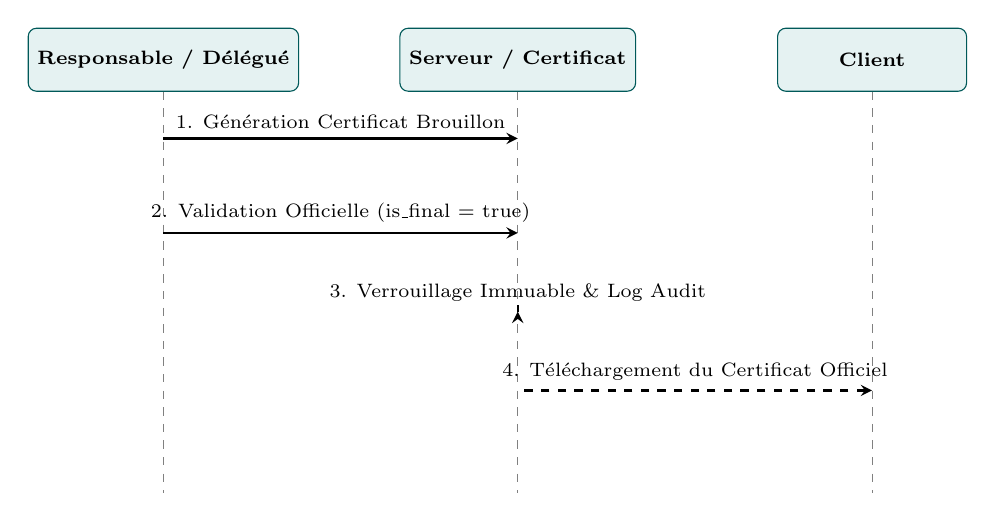
\begin{tikzpicture}[>=stealth,
    line/.style={dashed, color=gray},
    box/.style={draw=teal!70!black, fill=teal!10, rounded corners=3pt, minimum width=2.4cm, minimum height=0.8cm, align=center, font=\scriptsize\bfseries},
    msg/.style={->, thick, >=stealth, font=\scriptsize},
    reply/.style={<-, dashed, thick, >=stealth, font=\scriptsize}
]
\node[box] (m) at (0,0) {Responsable / D\'el\'egu\'e};
\node[box] (app) at (4.5,0) {Serveur / Certificat};
\node[box] (cl) at (9,0) {Client};

\draw[line] (m) -- (0,-5.5);
\draw[line] (app) -- (4.5,-5.5);
\draw[line] (cl) -- (9,-5.5);

\draw[msg] (0,-1) -- node[above] {1. G\'en\'eration Certificat Brouillon} (4.5,-1);
\draw[msg] (0,-2.2) -- node[above] {2. Validation Officielle (is\_final = true)} (4.5,-2.2);
\draw[msg] (4.5,-3.2) -- node[above] {3. Verrouillage Immuable \& Log Audit} (4.5,-3.2);
\draw[reply] (9,-4.2) -- node[above] {4. T\'el\'echargement du Certificat Officiel} (4.5,-4.2);
\end{tikzpicture}
